% PyTorch Conference North America 2026 poster (36 x 24 in, landscape)
% adapted from an unofficial NYU poster template
% a fork of https://github.com/anishathalye/gemini
% also refer to https://github.com/k4rtik/uchicago-poster



\documentclass[final]{beamer}

% ====================
% Packages
% ====================

\usepackage[T1]{fontenc}
 \usepackage[utf8]{luainputenc}
\usepackage{lmodern}
\usepackage[size=custom, width=91.44, height=60.96, scale=0.8]{beamerposter}
\usetheme{gemini}
\usecolortheme{pytorch}
\usepackage{graphicx}
\usepackage{booktabs}
\usepackage{tikz}
\usepackage{pgfplots}
\pgfplotsset{compat=1.14}
\usepackage{anyfontsize}
\usepackage{amssymb}   % \checkmark
\usepackage{qrcode}    % QR code to the repo

% grey box for numbers that are still being measured (none left)
\newcommand{\PH}{\textcolor{gray}{\rule{1.6em}{0.7em}}}

% ====================
% PyTorch Conference header band
% ====================

% Draw the official header artwork behind the Gemini headline
% (title, author, institute and logo), sized to fit it exactly.
\makeatletter
\let\geminiheadline\beamer@@tmpl@headline
\setbeamertemplate{headline}{%
  \setbox0=\vbox{\setbeamercolor*{headline}{fg=white}\geminiheadline}%
  \hbox{%
    \begin{tikzpicture}
      \node[inner sep=0pt, anchor=north west] at (0,0)
        {\includegraphics[width=\paperwidth, height=\dimexpr\ht0+\dp0\relax]{logos/pytorch_header_band.png}};
      \node[inner sep=0pt, anchor=north west] at (0,0) {\box0};
    \end{tikzpicture}%
  }%
}
\makeatother

% ====================
% Lengths
% ====================

% If you have N columns, choose \sepwidth and \colwidth such that
% (N+1)*\sepwidth + N*\colwidth = \paperwidth
\newlength{\sepwidth}
\newlength{\colwidth}
\setlength{\sepwidth}{0.025\paperwidth}
\setlength{\colwidth}{0.3\paperwidth}

\newcommand{\separatorcolumn}{\begin{column}{\sepwidth}\end{column}}

% ====================
% Title
% ====================

\title{Serving Interpretability Probes on Open Models}

\author{Aishwarya Ramasethu}

\institute[shortinst]{Prediction Guard}

% ====================
% Footer (optional)
% ====================

\footercontent{
  \href{https://github.com/aramasethu/probes-in-production}{GitHub: github.com/aramasethu/probes-in-production} \hfill
  PyTorch Conference North America 2026 \hfill
  \href{mailto:aishwarya.ramasethu@gmail.com}{aishwarya.ramasethu@gmail.com}}
% (can be left out to remove footer)

% ====================
% Logo (optional)
% ====================

% use this to include logos on the left and/or right side of the header:
% Left: PyTorch Conference logo
 \logoleft{\includegraphics[height=6cm]{logos/pytorch_conf_logo_white.png}}
% Right: funding agencies and other affilations
%\logoright{\includegraphics[height=7cm]{logos/NSF.eps}}
% ====================
% Body
% ====================

\begin{document}



\begin{frame}[t]
\begin{columns}[t]
\separatorcolumn

% ==================================================================
% COLUMN 1: why probes, and what serving hides
% ==================================================================
\begin{column}{\colwidth}

    \begin{block}{Probes in production}

    \textbf{Activation probes are small classifiers that read a model's hidden
    states. In 2026 they moved from research into frontier serving, and every
    public deployment is a safety screen.}

    \begin{table}
      \centering
      \begin{tabular}{@{}p{0.2\linewidth} p{0.25\linewidth} p{0.47\linewidth}@{}}
        \toprule
        \textbf{Who} & \textbf{Model} & \textbf{How it is served} \\
        \midrule
        Anthropic & Claude Opus 4.7--5.5 & Probe screens all traffic $\rightarrow$ classifier $\rightarrow$ block (cyber, prompt injection) \\
        Google DeepMind & Gemini 2.5 Flash, Gemini 4 Argon & Mid-layer attention probe on input $\rightarrow$ Gemini classifier (cyber, bio) \\
        OpenAI & GPT-5.6 Sol, Terra & During decode: pauses the stream $\rightarrow$ safety reasoner \\
        Goodfire & Kimi K3, GLM 5.3 & Probe in a \emph{private SGLang fork} $\rightarrow$ LLM judge (cyber) \\
        \bottomrule
      \end{tabular}
    \end{table}

    \begin{itemize}
      \item \textbf{Cascade:} the probe screens 100\% of traffic and escalates
        ${\sim}$5--8\% to an LLM classifier.
      \item \textbf{The math is free:} an all-layer probe costs ${\sim}$377K
        FLOPs/token vs.\ ${\sim}$8 GFLOPs/token for a 4B model.
      \item \textbf{The serving is not:} no lab publishes latency or how
        activations leave its engine; every decode-time blocking probe runs on
        an engine its operator owns or forked.
    \end{itemize}

    {\footnotesize Sources: Anthropic system cards \& arXiv 2601.04603; GDM
    arXiv 2601.11516 \& Gemini 4 blog; OpenAI GPT-5.6 system card; Goodfire
    (Oct 2026).}

  \end{block}

  \begin{block}{What optimized serving hides}

    \begin{figure}
      \centering
      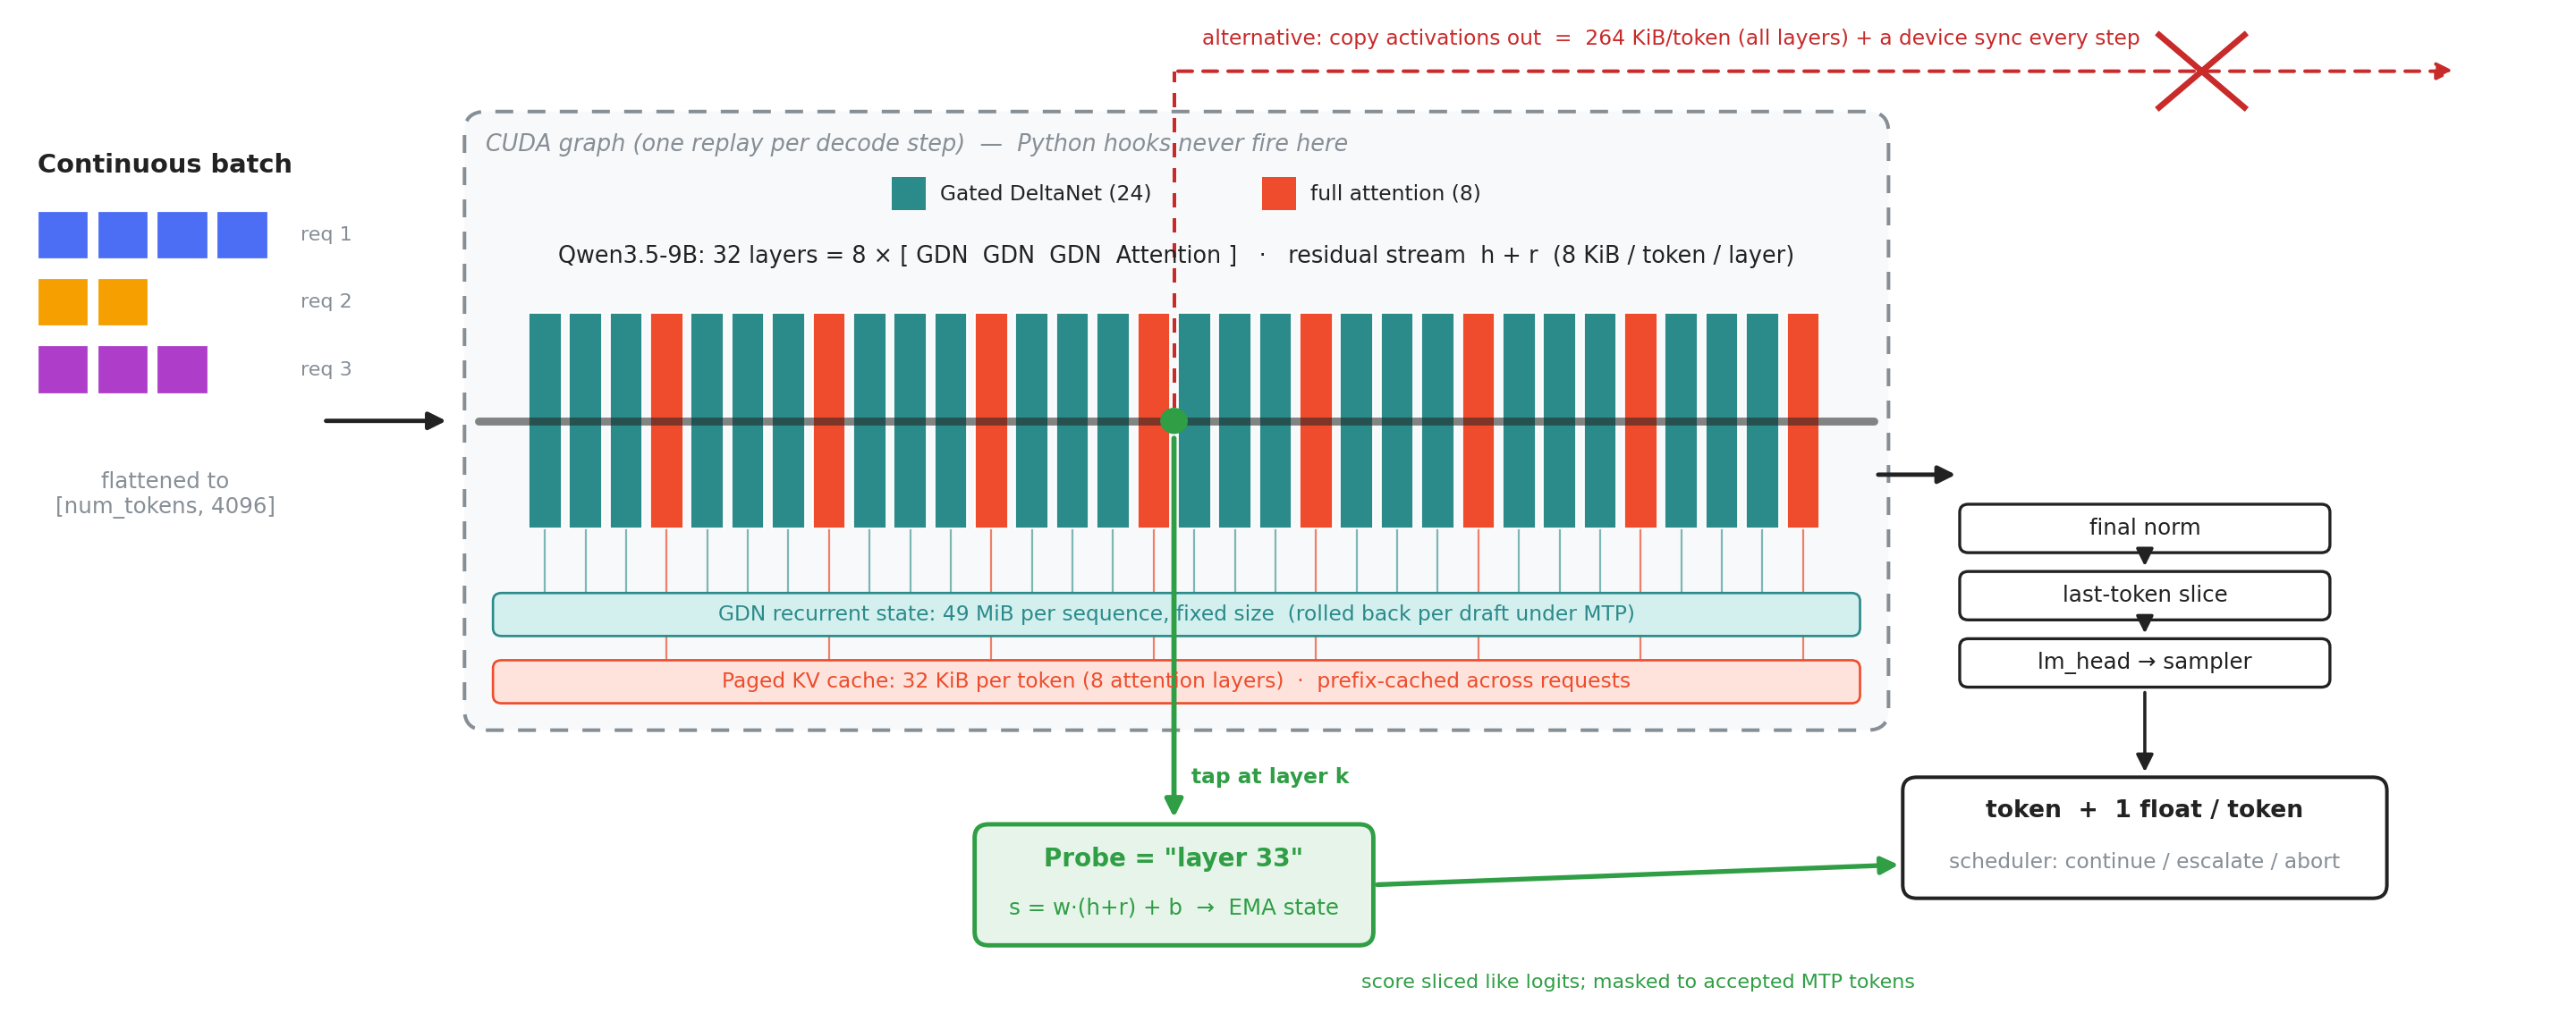
\includegraphics[width=0.96\linewidth]{figures/qwen35_decode_step.png}
    \end{figure}

    One decode step of \textbf{Qwen3.5-9B} (24 Gated DeltaNet + 8 attention
    layers) in vLLM / SGLang. Every optimization removes something a probe needs:

    \begin{itemize}
      \item \textbf{CUDA graphs:} decode is one graph replay, so Python hooks never fire.
      \item \textbf{Continuous batching:} activations are one flat
        \texttt{[num\_tokens, 4096]} tensor shared by all requests.
      \item \textbf{Fused add+RMSNorm:} the residual stream $h+r$ is never stored;
        it is overwritten in place (SGLang: not even summed until the next layer).
      \item \textbf{Prefix caching \& MTP speculation:} cached tokens produce no
        activations; drafted tokens may be rejected.
      \item \textbf{Final slice:} only last-token, final-layer states reach the output.
    \end{itemize}

    \textbf{Yet the probe is tiny:} 8 kFLOPs/token, about $10^{-6}$ of the forward pass.
    Copying out all 33 layers' activations instead costs 264\,KiB/token, 8$\times$ the KV cache.
    \textbf{Run the probe in the graph, as ``layer 33''.} Engines already manage a
    per-request recurrent state for GDN (49\,MiB/seq, rolled back under MTP); a probe's
    EMA is one more float.

\end{block}

\end{column}

\separatorcolumn
% ==================================================================
% COLUMN 2: can open engines do it, the math, code
% ==================================================================
\begin{column}{\colwidth}

  \begin{block}{Can probes be served out of the box in open serving frameworks?}

    \textbf{Not yet.} vLLM and SGLang can \emph{log} activations, but neither
    can run a mid-layer probe \emph{live during decode} with optimizations on.

    \begin{table}
      \centering
      \begin{tabular}{@{}p{0.32\linewidth} p{0.28\linewidth} p{0.32\linewidth}@{}}
        \toprule
        \textbf{Route} & \textbf{Status} & \textbf{Catch} \\
        \midrule
        Python hook on layer $k$ & CUDA graphs off only & Runs \textbf{0 of 128} steps with graphs on (measured) \\
        vLLM \texttt{extract\_hidden\_states} & Works, graphs on & Written to disk after the request; +15\% at batch 32 \\
        SGLang \texttt{return\_hidden\_states} & Works, graphs on & Final layer only \\
        Probe inside the graph & Not upstream & Shipped only in a private SGLang fork \\
        \bottomrule
      \end{tabular}
    \end{table}

    \textbf{What's missing:} an in-graph tap at layer $k$, a per-token score
    output, per-request probe state that survives prefix caching and MTP
    rollback, and a scheduler hook to abort or escalate.

    {\footnotesize Open proposals: vLLM \#59542, \#36998; SGLang \#43449, \#43450.
    Ours: SGLang \#45317 (bug), \#45318 (docs fix) (Oct 2026).}

  \end{block}

  % ---- the math, in the grey (example) block ----
  \begin{exampleblock}{The math of serving a probe}

    \heading{1. The probe is free}

    Linear probe on hidden size $d$ vs.\ a model with $N$ parameters (FLOPs and bytes per step):
    \[
      \frac{\text{probe}}{\text{model}} \approx \frac{2d}{2N}
      = \frac{4096}{9\times 10^{9}} \approx 5\times 10^{-7}
      \qquad \text{(Qwen3.5-9B)}
    \]

    \heading{2. Copying out costs waiting, not bandwidth}

    Normally the CPU prepares step $t{+}1$ while the GPU runs step $t$. A
    per-token \texttt{.cpu()} forces them to take turns:
    \[
      \text{overhead}
      = \frac{t_{\text{cpu}} + t_{\text{copy}} + t_{\text{gpu}}}{\max(t_{\text{cpu}},\, t_{\text{gpu}})} - 1
      \;\overset{t_{\text{gpu}} \ge t_{\text{cpu}}}{=}\;
      \frac{t_{\text{cpu}} + t_{\text{copy}}}{t_{\text{gpu}}}
    \]
    $t_{\text{copy}}$ is tiny (8\,KiB/token $\approx 0.3\,\mu$s over PCIe).
    Laptop: $27.6 \rightarrow 32.9$\,ms/token, i.e.\ $5.3/27.6 = 19\%$.
    \emph{Prediction: a faster GPU (smaller $t_{\text{gpu}}$) makes it worse.}

    \heading{3. Linear probes survive tensor parallelism}

    Across $P$ GPUs the tapped vector is the shared residual plus per-GPU
    partial outputs, $x = r + \sum_{i=1}^{P} o_i$, so
    \[
      p = \sigma\!\Big( w^\top r + b + \sum_{i=1}^{P} w^\top o_i \Big)
    \]
    Each GPU scores its own shard; all-reduce \emph{one scalar} per token
    instead of $d = 4096$. (The sigmoid comes after the sum, so this holds;
    an MLP probe with a hidden ReLU does not split this way.)

  \end{exampleblock}

  \begin{block}{Code, data and upstream work}

    \begin{columns}[c]
      \begin{column}{0.24\linewidth}
        \centering
        \qrcode[height=5.5cm]{https://github.com/aramasethu/probes-in-production}
      \end{column}
      \begin{column}{0.72\linewidth}
        \textbf{github.com/aramasethu/probes-in-production}\\[0.2em]
        {\small Laptop pipeline and GPU benchmarks (HF, vLLM 0.31.0, SGLang 0.5.21).
        Upstream: SGLang \#45317 (bug), \#45318 (docs fix).}
      \end{column}
    \end{columns}

  \end{block}

\end{column}

\separatorcolumn
% ==================================================================
% COLUMN 3: results (laptop + GPU in one table), then future work
% ==================================================================
\begin{column}{\colwidth}

  \begin{block}{Results}

    \heading{Laptop: the signal is real}

    \begin{figure}
      \centering
      \includegraphics[width=0.5\linewidth]{figures/layer_sweep.png}
    \end{figure}

    A linear probe on the last-token residual stream of Qwen2.5-1.5B reads
    truth from layer 13 on: \textbf{0.92 $\pm$ 0.005} (layer chosen in
    training; 10 entity-grouped splits, 312 statements). A bag-of-words
    baseline scores \textbf{0.50}. Factual recall is near-perfect; arithmetic
    is at chance.

    \heading{Laptop and GPU: what serving the probe costs}

    Extra time per token vs.\ the same setup without the probe (laptop, HF)
    or the engine's default with CUDA graphs on (vLLM, SGLang).

    \begin{table}
      \centering
      {\small
      \begin{tabular}{@{}l l c r r@{}}
        \toprule
        \textbf{Where} & \textbf{How the probe is served} & \textbf{Runs?} & \textbf{bs=1} & \textbf{bs=32} \\
        \midrule
        Laptop (MPS)   & probe on device                     & \checkmark               & $-0.6$\%            & -- \\
                       & probe via \texttt{.cpu()} per token & \checkmark               & $\mathbf{+19.1}$\%  & -- \\
        \midrule
        HF, L4         & probe inside the CUDA graph         & \checkmark               & $0.0$\%             & $0.0$\% \\
        \midrule
        SGLang, L4     & hook, CUDA graphs on                & $\times$ \textbf{0/128}  & $+0.1$\%            & $0.0$\% \\
                       & hook, CUDA graphs off               & \checkmark               & $\mathbf{+10.6}$\%$^*$ & $\mathbf{+8.3}$\%$^*$ \\
                       & \texttt{return\_hidden\_states}     & $\times$ final layer     & $+0.1$\%            & $+0.2$\% \\
        \midrule
        vLLM, L4       & hook, CUDA graphs on                & $\times$ \textbf{0/128}  & $0.0$\%             & $+0.1$\% \\
                       & hook, \texttt{enforce\_eager}       & \checkmark               & $\mathbf{+2.6}$\%   & $\mathbf{+2.6}$\% \\
                       & \texttt{extract\_hidden\_states}$^\dagger$ & after request   & $+2.0$\%            & $\mathbf{+14.6}$\% \\
        \bottomrule
      \end{tabular}}
    \end{table}

    \begin{itemize}
      \item \textbf{The probe is free where it runs in place:} on device
        ($-0.6$\%, within noise) or inside the CUDA graph (0.0\%).
      \item \textbf{Getting data out is the bill:} \texttt{.cpu()} per token
        +19\%; CUDA graphs off so a hook runs +3\% (vLLM) to +11\% (SGLang);
        vLLM \texttt{extract\_hidden\_states} +15\% at batch 32.
      \item \textbf{With CUDA graphs on, hooks never run} (0 of 128 passes).
        Every path that runs the probe matches HF's p(true) on 8/8 statements.
    \end{itemize}

    {\footnotesize Qwen2.5-1.5B-Instruct, probe at layer 15. Laptop: Apple
    Silicon, fp32, 48-token decode, 20 runs (95\% CIs $[-1.9, +2.2]$ and
    $[+17.7, +21.7]$). GPU: NVIDIA L4, bf16, 256 $\rightarrow$ 128 tokens,
    median of 3; vLLM 0.31.0, SGLang 0.5.21. $^*$Also turns off SGLang's overlap
    scheduler. $^\dagger$vs.\ vLLM's default on the same multiprocess engine.
    The L4 is memory-bound, so graph losses grow on faster GPUs.
    \textit{Caveat:} a probe trained on bare statements misfires in a chat
    template (AUC 0.95); train on the deployment format.}

  \end{block}

  \begin{block}{Future work}

    \begin{itemize}
      \item \textbf{More models, especially bigger ones.} Repeat these runs on
        larger models (e.g.\ Qwen3.5-9B, above; MoE) and on faster GPUs, where
        the cost model predicts leaving the graph costs more.
      \item \textbf{Different probes for different jobs.} Truthfulness is one;
        safety screens (cyber, prompt injection), hallucination, and attention
        or multi-layer probes like those in production. Nonlinear (MLP) probes
        do not split across tensor parallelism (math, part 3). Train each in the
        format it is served in.
    \end{itemize}

  \end{block}

  % References: the sources are cited inline above. Uncomment if you add poster.bib.
  % \begin{block}{References}
  %   \nocite{*}
  %   \footnotesize{\bibliographystyle{plain}\bibliography{poster}}
  % \end{block}

\end{column}

\separatorcolumn
\end{columns}
\end{frame}

\end{document}
